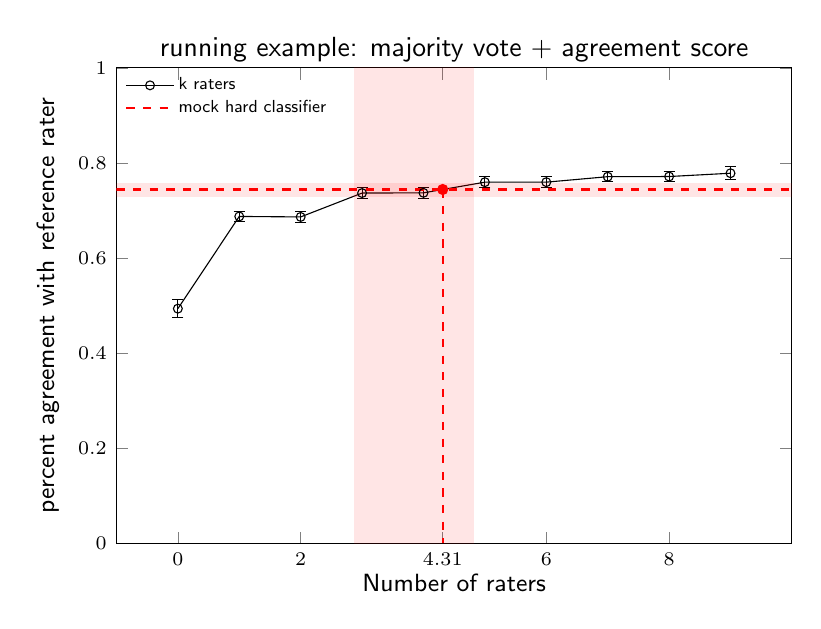
\begin{tikzpicture}
\sffamily
\begin{axis}[
title = {running example: majority vote + agreement score},
title style={align=center,yshift=-.1in},
legend style={font=\small,
	nodes={scale=0.7, transform shape},
	at={(0.0,1)},
	anchor=north west,
	draw=none,
	fill=none},
legend cell align={left},
width = 4.0in, height = 3.0in,
ylabel near ticks,
ylabel = {\small percent agreement with reference rater},
xlabel near ticks,
every tick label/.append style={font=\scriptsize},
xmin=-1,xmax=10,ymin=0,ymax=1,
xtick={0, 2, 4.313326656766923, 6, 8},
xlabel={\small Number of raters},
xlabel style = {yshift=0.05in},
yticklabel style={
		/pgf/number format/fixed,
		/pgf/number format/precision=5
},
scaled y ticks=false
]

\addplot[solid, mark=o, mark options={scale=.8}, black]
plot [error bars/.cd, y dir = both, y explicit]
table[y error index=2]{
0	0.4936	0.019520658682634584
1	0.6875111111111111	0.010261654468840087
2	0.6865055555555554	0.010839044133954645
3	0.7367142857142852	0.01131425244748685
4	0.7371666666666667	0.011153490549764
5	0.759613953488372	0.011382690433086817
6	0.7596267605633801	0.011300520437997008
7	0.7711222222222223	0.010934686183189823
8	0.7714666666666669	0.011067864271457561
9	0.7784	0.013296606786426968

};
\addlegendentry{k raters}



\addplot[mark=none, red, dashed, thick, samples=2, domain=-1:31] {0.7441999999999999};
\addlegendentry{mock hard classifier}

\draw [red, fill=red, opacity=0.1] (axis cs:-1,0.7297499999999999) rectangle (axis cs:31,0.7563500000000001);



\addplot[mark=*, mark options={scale=.8}, red, thick]
    table[]{
        4.313326656766923	0.7441999999999999
    };

\addplot[mark=none, red, dashed, thick, samples=2, domain=-1:31] coordinates {(4.313326656766923,0.7441999999999999) (4.313326656766923,0)};

\draw [red, fill=red, opacity=0.1] (axis cs:2.881321831139446,-1) rectangle (axis cs:4.808570585542146,1);


\end{axis}
\end{tikzpicture}